\documentclass[12pt]{article}

\usepackage{fancyhdr}
\usepackage{extramarks}
\usepackage{amsmath}
\usepackage{amsthm}
\usepackage{amssymb}
\usepackage{amsfonts}
\usepackage{tikz}
\usepackage[plain]{algorithm}
\usepackage{algpseudocode}
\usepackage{graphicx}

\usetikzlibrary{automata,positioning}

%
% Basic Document Settings
%

\topmargin=-0.45in
\evensidemargin=0in
\oddsidemargin=0in
\textwidth=6.5in
\textheight=9.0in
\headsep=0.25in

\linespread{1.1}

\pagestyle{fancy}
\lhead{\hmwkAuthorName}
\chead{\hmwkClass\ \hmwkTitle}
\rhead{\firstxmark}
\lfoot{\lastxmark}
\cfoot{\thepage}

\renewcommand\headrulewidth{0.4pt}
\renewcommand\footrulewidth{0.4pt}

\setlength\parindent{0pt}

%
% Create Problem Sections
%

\newcommand{\enterProblemHeader}[1]{
    \nobreak\extramarks{}{Problem \arabic{#1} continued on next page\ldots}\nobreak{}
    \nobreak\extramarks{Problem \arabic{#1} (continued)}{Problem \arabic{#1} continued on next page\ldots}\nobreak{}
}

\newcommand{\exitProblemHeader}[1]{
    \nobreak\extramarks{Problem \arabic{#1} (continued)}{Problem \arabic{#1} continued on next page\ldots}\nobreak{}
    \stepcounter{#1}
    \nobreak\extramarks{Problem \arabic{#1}}{}\nobreak{}
}

\setcounter{secnumdepth}{0}
\newcounter{partCounter}
\newcounter{homeworkProblemCounter}
\setcounter{homeworkProblemCounter}{1}
\nobreak\extramarks{Problem \arabic{homeworkProblemCounter}}{}\nobreak{}

%
% Homework Problem Environment
%
% This environment takes an optional argument. When given, it will adjust the
% problem counter. This is useful for when the problems given for your
% assignment aren't sequential. See the last 3 problems of this template for an
% example.
%
\newenvironment{homeworkProblem}[1][-1]{
    \ifnum#1>0
        \setcounter{homeworkProblemCounter}{#1}
    \fi
    \section{Problem \arabic{homeworkProblemCounter}}
    \setcounter{partCounter}{1}
    \enterProblemHeader{homeworkProblemCounter}
}{
    \exitProblemHeader{homeworkProblemCounter}
}

%
% Homework Details
%   - Title
%   - Date
%   - Class
%   - Instructor
%   - Author
%

\newcommand{\hmwkTitle}{Homework\ \#8}
\newcommand{\hmwkDate}{2017-04-29}
\newcommand{\hmwkClass}{MATH6222}
\newcommand{\hmwkClassInstructor}{Instructor: Dr. David Smyth}
\newcommand{\hmwkTutor}{Tutor: Mark Bugden (Wednesday 1-2pm)}
\newcommand{\hmwkAuthorName}{\textbf{Rui Qiu u6139152}}

%
% Title Page
%

\title{
    \vspace{2in}
    \textmd{\textbf{\hmwkClass:\ \hmwkTitle}}\\
    \normalsize\vspace{0.1in}\small{\hmwkDate}\\
    \vspace{0.1in}\large{\textit{\hmwkClassInstructor}}\\
    \vspace{0.1in}
    	\large{\textit{\hmwkTutor}}
    \vspace{3in}
}

\author{\hmwkAuthorName}
\date{}

\renewcommand{\part}[1]{\textbf{\large Part \Alph{partCounter}}\stepcounter{partCounter}\\}

%
% Various Helper Commands
%

% New QED symbol
\renewcommand{\qedsymbol}{$\blacksquare$}

% Useful for algorithms
\newcommand{\alg}[1]{\textsc{\bfseries \footnotesize #1}}

% For derivatives
\newcommand{\deriv}[1]{\frac{\mathrm{d}}{\mathrm{d}x} (#1)}

% For partial derivatives
\newcommand{\pderiv}[2]{\frac{\partial}{\partial #1} (#2)}

% Integral dx
\newcommand{\dx}{\mathrm{d}x}

% Alias for the Solution section header
\newcommand{\solution}{\textbf{\large Solution}}

% Probability commands: Expectation, Variance, Covariance, Bias
\newcommand{\E}{\mathrm{E}}
\newcommand{\Var}{\mathrm{Var}}
\newcommand{\Cov}{\mathrm{Cov}}
\newcommand{\Bias}{\mathrm{Bias}}

\begin{document}

\maketitle

\pagebreak

\begin{homeworkProblem}
\textit{Variations on Wilson's Theorem}

(a) Prove that if $p$ is prime, $2(p-3)!+1$ is divisible by $p$.\\

\textbf{Proof:} First we claim that $p\geq 3$, otherwise, $p-3<0$. Recall Wilson's Theorem which states 

\[(p-1)!\equiv -1\mod p\].

We also know that $(p-1)!=(p-1)\cdot (p-2)\cdot (p-3)!$. Since we've already claim that $p\geq 3$, then $(p-1)\cdot (p-2)\equiv (-1)\cdot (-2)\equiv 2\mod p$.\\

Therefore, $(p-1)!\equiv 2(p-3)!\equiv -1\mod p$. In other words, $2(p-3)!+\equiv 0 \mod p$, $2(p-3)!+1$ is divisible by $p$.

\qed\\

(b) Prove that if $p$ divides $(p-1)!+1$, then $p$ is prime. (This is the converse to Wilson's Theorem.)\\

\textbf{Proof:} We try to prove the contrapositive of this statement: \textit{If $p$ is not prime, then $p$ does not divide $(p-1)!+1$.}\\

Since $p$ is not a prime now, suppose $p=m\cdot t$ where $m,t$ are two positive integers smaller than $p$. Obviously, $m,t$ included in the factorial $(p-1)!=1\cdot 2\cdot 3\cdots (p-2)\cdot (p-1)$. Therefore,

\[
\begin{split}
	(p-1)!&\equiv 0 \mod (m\cdot t)\\
	(p-1)!&\equiv 0 \mod p\\
	(p-1)!&\not\equiv -1 \mod p	
\end{split}
\]

So we proved the contrapositive of our desired statement. We are done.

\qed
\end{homeworkProblem}

\begin{homeworkProblem}
\textit{An important equivalence relation in analysis}. Fix a function $f:\mathbb{R}\rightarrow\mathbb{R}$, and let $O(f)$ denote the set of functions $g:\mathbb{R}\rightarrow\mathbb{R}$ for which there exists positive constants $c$ and $a$ such that $|g(x)|\leq c|f(x)|$ for all $x>a$. Now let $S$ denote the set of all functions from $\mathbb{R}$ to $\mathbb{R}$, and define a relation $R$ on $S$ by setting $(g,h)\in R$ if and only if $g-h\in O(f).$ Prove that $R$ is an equivalence relation.\\

\textbf{Proof:}
\begin{itemize}
	\item \textbf{Reflexive property:} Let $c,a$ be arbitrary positive constants, we always have $|g(x)-g(x)|=0\leq c|f(x)|, \forall x>a$. In fact, this holds for any $x\in\mathbb{R}$. Therefore $(g,g)\in R$.
	\item \textbf{Symmetric property:} Suppose we have $(g,h)\in\ R$ then we get $\exists\ c>0, a>0, x>a, |g(x)-h(x)|\leq c|f(x)|$. It not hard to see that $\exists\ c>0, a>0, x>a, |h(x)-g(x)|\leq c|f(x)|$, for the same constants $c,a$. Therefore, $(h,g)\in R$.
	\item \textbf{Transitive property:} Suppose $(g,h)\in R$ for some constants $c, a$ and $(h, i)\in R$ for some constants $c', a'$. Use triangle inequality we get:\\
	\[
		\begin{split}
			|g(x)-i(x)|&=|g(x)-h(x)+h(x)-i(x)|\\
			&\leq |g(x)-h(x)|+|h(x)-i(x)|\\
			&\leq c|f(x)| + c'|f(x)|\\
			&=(c+c')|f(x)|
		\end{split}
	\]
	Now for $(g,i)$ we can just fix two positive constants $c'' = c+c'$ and $a'' = \max(a, a')$, then $(g,i)\in R$.
\end{itemize}

Since we have proved the three properties of an equivalence relation, so $R$ is an equivalence relation.
\qed
\end{homeworkProblem}

%\begin{homeworkProblem}
%\textit{Linear Equations in Modular Arithmetic.} Let $n\in\mathbb{N}$, let $a, b\in\mathbb{Z}$, and set $d=\gcd(a,n)$. Prove that the equation
%
%\[ax\equiv b\mod n\]
%
%has a solution if and only if $d|b$. Furthermore, prove that when $d|b$, there are exactly $d$ distinct congruence classes of solutions.
%\end{homeworkProblem}

\begin{homeworkProblem}[4]
\textit{Euler's Theorem.} This is a generalization of Fermat's little theorem to nonprime moduli. Let $\phi(n)$ denote the number of integers less than $n$ which are relatively prime to $n$. For example, $\phi(10)=4$ since $1,3,7,9$ are relatively prime to $10$. Prove that if $a\in\mathbb{Z}$ is relatively prime to $n$, then

\[a^{\phi(n)}\equiv 1\mod n\]

Hint: Consider the set $\{ia: 1\leq i\leq n-1, \gcd(i,n)=1\}$ and mimic our proof of Fermat's Little Theorem.\\

\textbf{Proof:} Let $S=\{ia: 1\leq i\leq n-1, \gcd(i,n)=1\}=\{i_1,i_2,\dots, i_{\phi(n)}\}$.

Then another set $aS=\{ai_1,ai_2,\dots,ai_{\phi(n)}\}$. Since we have $a, n$ are relatively prime, $\gcd(a,n)=1$. By the fact that $a$ permutes $i_l$, i.e. if $ai_j\equiv ai_k \mod n$ then $j=k$, then the sets $S$ and $aS$ are considered as sets of congruence classes modulo $n$, which are identical. Hence, we could have

\[
\begin{split}
	ai_1\cdot ai_2\cdots ai_{\phi(n)}&\equiv i_1\cdot i_2\cdots i_{\phi(n)}\mod n\\
	a^{\phi(n)}&\equiv 1\mod n
\end{split}
\]

\qed
\end{homeworkProblem}

\begin{homeworkProblem}[5]
\textit{Functional Digraphs from Modular Arithmetic.} Define $f$ and $g$ from $\mathbb{Z}_n$ to $\mathbb{Z}_n$ by

\[
\begin{split}
	f(x)&\equiv x+a \mod n\\
	g(x)&\equiv ax \mod n
\end{split}
\]

(a) Draw the functional digraphs of $f$ and $g$ in the cases $(n,a)=(19,4)$ and $(n,a)=(20,4)$.\\

\textbf{Solution:}

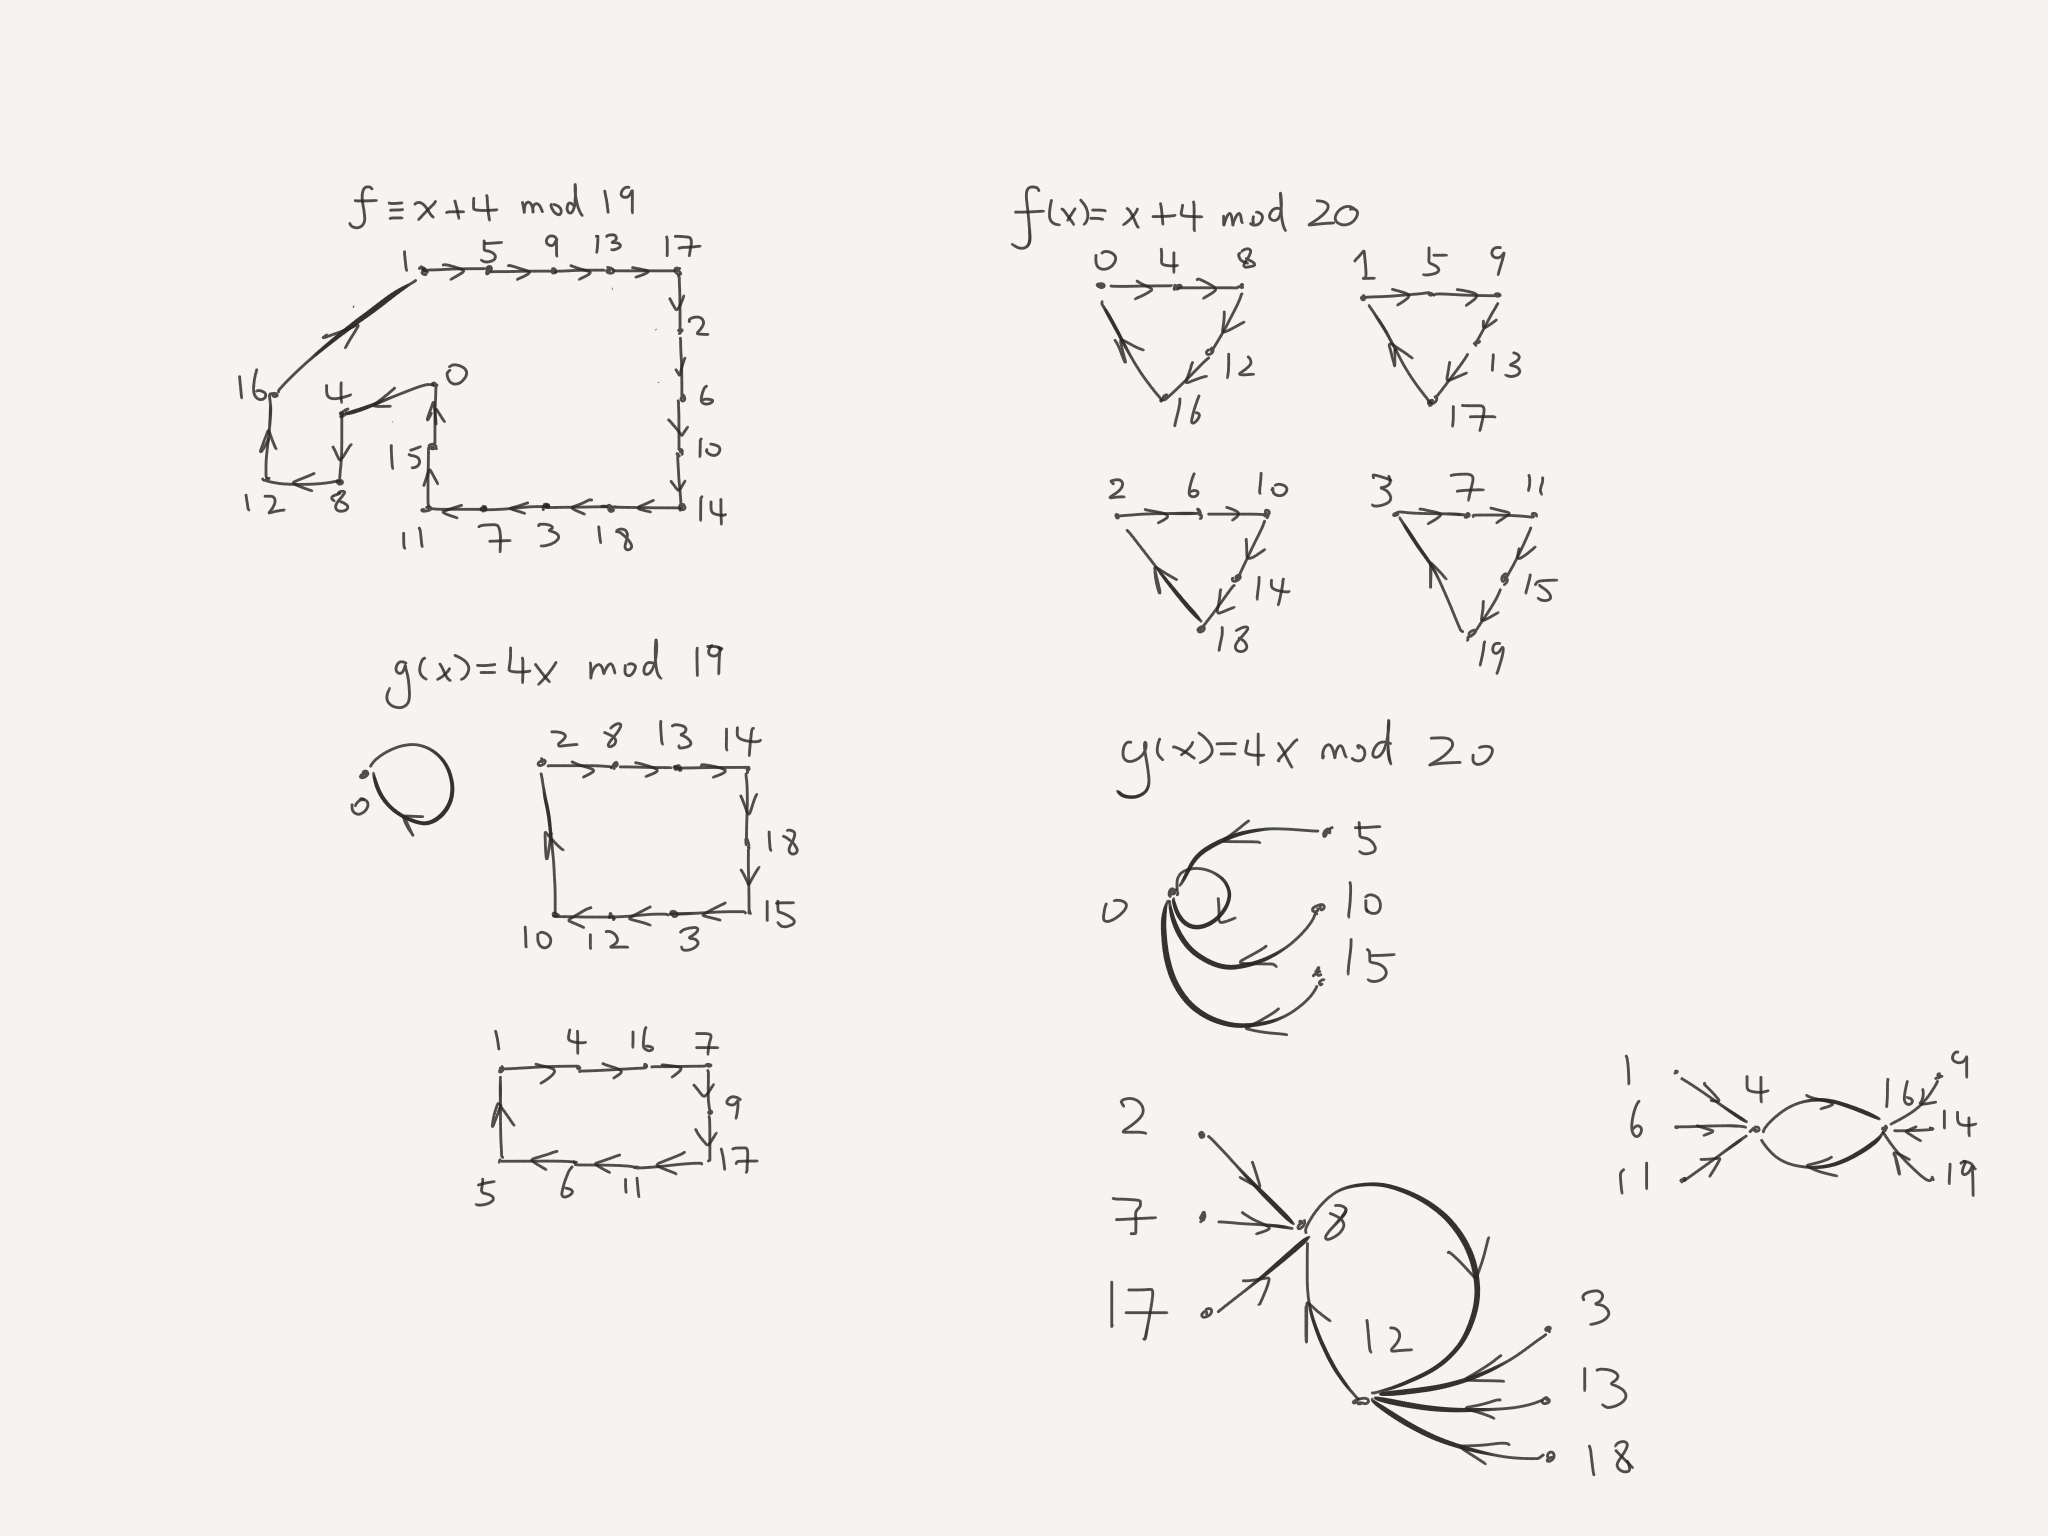
\includegraphics[width=\textwidth]{images/digraph}

(b) Give a complete description of the functional digraph of $f$ in terms of $a$ and $n$.\\

\textbf{Solution:} The functional digraph of $f$ is a collection of $\gcd(n,a)$ cycles with length $\frac{n}{\gcd(n,a)}$.\\

In our case, when $n=19, a=4, \gcd(19,4)=1$, the functional digraph of $f$ is a cycle of length $19/1=19$. When $n=20, a=4,\gcd(20,4)=4$, the functional digraph of $f$ is 4 cycle of length $20/4=5$.\\

The reasoning is we would like to add multiple $a$'s to a number in order to get a multiple of $n$. Such minimum multiple of $n$ is the least common multiple of $n$ and $a$, which satisfies

\[\text{lcm}(n,a)=\frac{na}{\gcd(n,a)}\]

Also need to divide $\text{lcm}(n,a)$ by the ``step-length'', which is $a$, so the cycle length is $\frac{na}{a\cdot\gcd(n,a)}= \frac{n}{\gcd(n,a)}$.\\

(c) Describe a property of the digraph of $g$ which is true whenever $n$ is prime and false whenever $n$ is not prime.\\

\textbf{Solution:} When $n$ is prime, $g$ consists of a cycle of length $1$ and other cycles of equal length.\\

In our case, when $n=19$, $g$ contains a cycle from $0$ to $0$ and two cycles of length $9$. But this fails when $n=20$, which is not a prime.

\end{homeworkProblem}

%
% Non sequential homework problems
%

% Jump
%\begin{homeworkProblem}[5]

%\end{homeworkProblem}

\end{document}
